\documentclass{article}
\PassOptionsToPackage{numbers,sort&compress}{natbib}
\usepackage[preprint]{neurips_2025}
\usepackage[T1]{fontenc}
\usepackage[utf8]{inputenc}
\usepackage{hyperref}
\usepackage{url}
\usepackage{booktabs}
\usepackage{amsmath}
\usepackage{graphicx}
\usepackage{xcolor}
\makeatletter
\renewcommand{\@noticestring}{Technical report, Predictive AI Evaluation Competition (PAIEC) 2026.}
\makeatother

\title{Knowing the Model Is Worth Six Answers:\\ Language-Model Priors for Predicting AI Responses\\ on New Benchmarks}

\author{%
  Siwei Shan\thanks{Equal contribution.}\\
  NLPQuant AI Inc.\\
  \And
  Sunny Yang\footnotemark[1]\\
  University of Illinois Urbana-Champaign\\
  \texttt{guangy4@illinois.edu}
  \And
  Weiyan Zhao\\
  NLPQuant AI Inc.\\
}

\begin{document}
\maketitle

\begin{abstract}
How much evidence does it take to predict how an AI system answers a new benchmark? Most of the error comes before the system has answered anything, when the predictor does not know how strong it is. We find that a language model's knowledge of the system closes much of that gap. Given the system's name and settings and a few of the benchmark's items, Claude Opus estimates its accuracy as well as about six of the system's own answers would. Hiding the system's identity removes almost all of this value, and naming the benchmark adds nothing measurable. We use the estimate as a Beta prior in a predictor that pools labels across systems. On identical simulated draws it lowers Brier ALC by 0.007 with one system per benchmark and by 0.008 with four, improving 80\% and 93\% of draws. On benchmarks held out from all development it does nothing for unnamed systems and helps on five of eight benchmarks with named ones. Online, it cut the excess error before the first label from 0.119 to about 0.03. Code, cached model outputs and a script for every table are released.
\end{abstract}

\section{Introduction}
\label{sec:intro}

The Predictive AI Evaluation Competition asks for the probability that a subject (a model under a given configuration) answers an item correctly, on benchmarks the predictor has never seen, after it reveals 0, 1, 3, 7, 15 and 31 of its own answers. The score is the Brier area under that learning curve (ALC), and budgets 0 to 3 carry half of its weight. The competition's question is how much evidence prediction needs. At the start the answer is: more than the subject has given. With one subject on a benchmark and no labels, a predictor cannot tell a model that answers nearly everything from one that answers half.

We find that a language model already holds much of that evidence. Asked how often a named model answers items like the ones shown, Claude Opus is as informative as about six of the model's own answers, while priors from the model's metadata or its accuracy on other benchmarks are no better than guessing one half. The value comes from knowing which model it is: hidden behind an anonymous description, the estimate is barely better than a constant.

Our contributions:
\begin{itemize}
\item \textbf{The finding, measured in the competition's currency} (Section~\ref{sec:prior}): the number of revealed answers a language model's estimate replaces, how it depends on the subject's identity, and where it stops helping.
\item \textbf{Controlled evidence} (Section~\ref{sec:ablate}): the submitted predictor on identical simulated draws with each language-model term switched off, with one and with four subjects per benchmark, and on 15 benchmarks used in no development step.
\item \textbf{Lessons for the competition} (Section~\ref{sec:online}): three runs of the same package scored 0.130 to 0.181, almost entirely because of the draw. We show how to read formative scores despite this, and how the platform's worker processes affect language-model submissions.
\end{itemize}

\paragraph{Related work.} The organisers' Bayesian Linguistic Evaluator baseline also starts from a language model's estimate, but it asks for every target response separately and revises the estimate inside the prompt. We ask once per subject and benchmark for an aggregate accuracy, update it numerically with labels pooled across subjects, and calibrate item ratings by regression on the revealed labels. Language models have also been asked to forecast a benchmark score from a description of the task \cite{park2025}, and a model's missing scores can be filled in from its scores on other benchmarks \cite{zeng2026}. Both predict one aggregate score per model and benchmark. We use such a forecast as the prior of an item-level predictor. Methods that predict performance from few items usually assume items calibrated on many models, through item response theory \cite{polo2024tiny,hofmann2025}, anchor items \cite{vivek2023} or amortised item models \cite{truong2025}. On a held-out benchmark no such calibration exists. In educational measurement terms the task is a Rasch-type model \cite{rasch1960,lord1980} fitted online with very few responses per examinee, as in computerised adaptive testing \cite{vanderlinden2010}, and the subject prior is the collateral information that sets an examinee's ability prior before any responses \cite{mislevy1987}. Here the background variables are a model's name and settings, and a language model maps them to an expected score.

\section{Task and scoring}
\label{sec:task}

For each subject--benchmark pair, the items are split 50/50 into an acquisition pool and an evaluation pool. Acquisition items stream past in random order, and an acquisition function decides whether to reveal each one, up to 31 reveals. Predictions on the evaluation pool are scored at budgets $b \in \{0,1,3,7,15,31\}$ with weights $0.1, 0.2, 0.2, 0.2, 0.2, 0.1$, and the ALC is averaged equally over pairs. The labels a program sees are pooled across all sampled pairs, and the rules state that ``the submitted program may use the attributes and acquired labels supplied through the evaluation interface to adapt during evaluation''. Because the split is drawn separately for each pair, an item one subject reveals is often in another subject's evaluation pool. The program sees each item's text and features and each subject's attributes, never reference answers. Formative evaluation on Codabench is capped at 1{,}000 subject--item cells, about 100 items per pair.

\section{Method}
\label{sec:method}

No parameters are fitted to the training responses. The subject prior's calibration examples and its two constants (shrinkage 0.75 and $k_0=4$) come from the prior-evaluation pairs, and the remaining settings (such as $k=8$ and the ridge penalty) were chosen in simulation on the 12 simulation benchmarks, which therefore serve as development data. Every other quantity is estimated at prediction time from the labels revealed so far in the evaluation, on the target benchmark where it has enough of them and across benchmarks otherwise, as for the rating slope below.

\paragraph{Subject prior.} \label{sec:prior-method} We ask Claude Opus~5.5 what percentage of the benchmark's items the subject answers correctly, given up to eight sample items (each cut to 600 characters) and the subject's attributes: name, provider, release date, harness and reasoning effort. Eight solved examples from public training benchmarks, each with a model name, two sample items and that model's true accuracy, precede the question and fix the scale. The estimate $q_s$ is shrunk toward one half, $m_s = 0.5 + 0.75\,(q_s - 0.5)$, used directly at budget 0 and as a Beta prior with $k_0=4$ pseudo-counts once the subject's own labels $R_s$ arrive:
\begin{equation}
\hat\mu_s = \frac{\sum_{j \in R_s} y_{sj} + k_0\, m_s}{|R_s| + k_0}.
\end{equation}
A worker asks first from the sample items it has seen, often just one, and once more when eight are available. It stops asking once the subject has eight labels of its own. If Opus gives no number, the predictor asks Claude Sonnet~5.5 and then Claude Haiku~5.5.

\paragraph{Pooling across subjects.} When other subjects have at least ten labels on the benchmark, subject $s$'s rate is shrunk toward their success rate $\bar y_{-s}$ with $k=8$ pseudo-counts, $\hat\mu_s = (\sum_{j \in R_s} y_{sj} + k\,\bar y_{-s})/(|R_s| + k)$, and the two subjects' language-model estimates shift the pooled rate by half their difference. Deviations are measured against item-level predictions rather than the benchmark mean, so a correct answer on a hard item raises $\hat\mu_s$ more than one on an easy item.

\paragraph{Item level.} Three terms move a prediction away from $\hat\mu_s$. (i) When other subjects have answered the target item itself, one Newton step on the item's logit shift under a Rasch model with prior variance $\tau^2=1$:
\begin{equation}
\operatorname{logit}\hat p_{sj} \leftarrow \operatorname{logit}\hat p_{sj} + \frac{\sum_{s' \neq s} (y_{s'j} - \hat p_{s'j})}{\sum_{s' \neq s} \hat p_{s'j}(1-\hat p_{s'j}) + 1/\tau^2}.
\end{equation}
(ii) The similarity-weighted mean residual of the 30 nearest revealed items, by cosine similarity of hashed character $n$-grams. (iii) A difficulty rating: Claude Opus~5.5 gives the probability that a typical current model answers the item correctly, and residuals are regressed on the standardised rating with a ridge penalty, so the rating is calibrated on the fly to the subjects at hand. Given each pair's true accuracy, Opus ratings lower the item-level Brier score on 70{,}563 responses from 11 simulation benchmarks from 0.1508 to 0.1387, against 0.1440 for Claude Haiku~5.5, with the slope picked on the same responses (\texttt{src/item\_signal\_oracle.py}).

\paragraph{Acquisition.} The acquisition function reveals an item only if no subject has revealed it yet on this benchmark, and always reveals when the remaining items are no more than the remaining budget. This maximises the number of evaluation items that carry an exact-item label from someone else. The rule looks only at which items were revealed, never at outcomes, so pooled rates stay unbiased.

\paragraph{Implementation.} The platform runs predictions in several worker processes and recreates them at every budget, and workers need not share memory or disk. Every subject prior is written to several candidate cache directories and read from any of them. A failed rating is not written to disk, so other workers retry it, and a failed prior call can be retried once its lock is three minutes old. Calls retry on rate limits, and hard caps per worker (150 prior calls, 300 item ratings) bound the cost. When a cap is hit or no key is present, the predictor drops the language-model terms and runs on pooled labels alone. One formative run costs about \$10 to \$15.

\section{What the language model knows}
\label{sec:prior}

We evaluated the prior on 87 subject--benchmark pairs from 25 public training benchmarks against each pair's true accuracy, leaving out the eight pairs that serve as calibration examples. Each estimate saw five sample items cut to 600 characters. To express the error in the competition's currency, we find the number of the subject's own labels $n$ at which a Laplace estimate $(k+1)/(n+2)$ has the same mean squared error, averaged over the same pairs with $k \sim \mathrm{Binomial}(n, \text{accuracy})$.

\begin{table}[t]
\centering
\caption{Subject prior quality on held-out training pairs. ``Labels'' is the number of the subject's own answers a Laplace estimate needs to match the prior's mean squared error. Model rows use the 71 pairs on which all three models gave a number. Every estimate used the deployed prompt with five sample items. The deployed row uses all 79 pairs, with the shrinkage chosen leave-one-benchmark-out, and a 90\% interval from a bootstrap over benchmarks.}
\label{tab:prior}
\small
\begin{tabular}{lcccc}
\toprule
Prior & Pairs & RMSE & Correlation & Labels \\
\midrule
Constant 0.5 & 71 & 0.217 & -- & 0 \\
Claude Haiku~5.5 & 71 & 0.185 & 0.63 & 3 \\
Claude Sonnet~5.5 & 71 & 0.142 & 0.76 & 7 \\
Claude Opus~5.5 & 71 & 0.141 & 0.76 & 7 \\
\midrule
Deployed: Opus, then Sonnet, then Haiku & 79 & 0.153 [0.118, 0.184] & 0.69 & 6 [3, 13] \\
Opus, calibration benchmarks removed & 48 & 0.149 & 0.78 & 6 \\
Opus, simulation benchmarks removed & 35 & 0.131 & 0.62 & 10 \\
\bottomrule
\end{tabular}
\end{table}

Table~\ref{tab:prior} shows the result. Opus and Sonnet estimate accuracy with an RMSE of 0.14, each worth about seven revealed answers, and Haiku is worth three. Opus gave no number on the eight pairs of two benchmarks, where the deployed predictor falls back to Sonnet and then Haiku. With that fallback and the shrinkage chosen leave-one-benchmark-out, the deployed prior is worth six labels, removing every benchmark that supplied a calibration example still leaves Opus worth six, and on the 35 pairs outside the 12 simulation benchmarks, which served as development data, it is worth ten. Cheap priors that use no language model did not work. Rank correlations between true accuracy and priors from the model's name, its release date or its accuracy on other benchmarks ranged from $-0.5$ to $0.46$ across benchmarks, and using the subject's accuracy on other training benchmarks as its budget-0 prediction scored 0.252, against 0.250 for a constant one half.

The value of a prior depends on the subjects. When accuracy sits near 0 or 1, a few labels already pin it down, and the same prior error is worth fewer labels. Many online subjects answered nearly every item, and there the prior was worth two to three labels (Section~\ref{sec:online}).

\paragraph{Estimating or remembering?} A language model might recall published scores rather than estimate them. We tested this on the same 71 pairs with two variants of the deployed Opus prompt. Hiding the subject's identity (name, provider, release date and model identifier) raises the RMSE from 0.141 to 0.211, close to the constant's 0.217, so the estimate depends on knowing the model. Naming the benchmark, which the deployed prompt never does, changes it from 0.141 to 0.136 (90\% benchmark-bootstrap interval for the change $-0.021$ to $+0.010$). If the estimates came from retrieving a published score for this model on this benchmark, the name should help, and it gave no measurable gain. These tests cannot exclude that the model recognises a benchmark from its items and recalls a score that way. The online benchmarks, from the organisers' held-out pool, point the same way: the prior's error there was 0.16 to 0.19 (Section~\ref{sec:online}). We release the estimates for all 87 training pairs (\texttt{data/llm/prior\_estimates.csv}) as a starting prior for other predictors.

\section{Controlled evidence}
\label{sec:ablate}

Online versions differ in their draws as well as their code. To compare components on identical draws, we ran the submitted predictor in an online-regime simulator: nine pairs over seven of the 12 simulation benchmarks per draw, mostly one subject per benchmark, 120 items per benchmark and the subject attributes as the online inputs give them, over 90 draws (three seeds of 30). Every draw starts from a fresh state, as a new evaluation does. Item ratings come from cached Opus ratings. Subject priors are real Opus calls with the deployed prompt, cached so that every variant sees the same estimates (641 calls, about \$10). We then switched the subject prior and the item ratings off in turn, and added a smoothed baseline that predicts $(k+1)/(n+2)$ from the subject's own labels.

\begin{table}[t]
\centering
\caption{The submitted predictor on identical simulated draws (90 draws). Differences are paired over draws, mean $\pm$ standard error, against the variant with both language-model terms off.}
\label{tab:ablate}
\small
\begin{tabular}{lcccc}
\toprule
Variant & ALC & $B_0$ & Difference & Better in \\
\midrule
Laplace estimate on own labels & 0.2020 & 0.250 & $+0.0008 \pm 0.0002$ & 20\% of draws \\
Neither term & 0.2012 & 0.250 & -- & -- \\
Item ratings only & 0.1992 & 0.244 & $-0.0020 \pm 0.0004$ & 68\% of draws \\
Subject prior only & 0.1941 & 0.221 & $-0.0071 \pm 0.0009$ & 80\% of draws \\
Both (submitted) & \textbf{0.1924} & 0.216 & $-0.0088 \pm 0.0010$ & 83\% of draws \\
\bottomrule
\end{tabular}
\end{table}

Table~\ref{tab:ablate} shows the result. With mostly one subject per benchmark, the predictor without its language-model terms is barely better than the smoothed baseline, so nearly all of the gain comes from those terms, and the subject prior is the larger of them. With item ratings on, adding it lowers the ALC by $0.0068 \pm 0.0009$ and helps in 80\% of draws. With the prior on, item ratings add $0.0017 \pm 0.0004$. The prior acts where the method predicts: Brier at budget 0 falls from 0.244 to 0.216, and the gap closes by budget 7, once the subject's own labels dominate. The simulated gain is smaller than the online 0.017 from Table~\ref{tab:online}, which compares different draws and is the less controlled of the two.

\begin{table}[t]
\centering
\caption{The subject prior across regimes, paired over identical simulated draws. ``Prior'' is the ALC difference from switching the prior on (negative is better), mean $\pm$ standard error over draws. The held-out benchmarks were used in no development step. Their item ratings are off in both arms, and their difference is reported per benchmark group.}
\label{tab:regimes}
\small
\begin{tabular}{lcccc}
\toprule
Regime & Draws & Pairs & Prior & Better in \\
\midrule
One subject per benchmark (mostly) & 90 & 9 & $-0.0068 \pm 0.0009$ & 80\% \\
Four subjects per benchmark & 30 & 28 & $-0.0076 \pm 0.0008$ & 93\% \\
Held-out, named subjects (8 bench.) & 90 & -- & $-0.0011$ & 5 of 8 bench. \\
Held-out, unnamed subjects (7 bench.) & 90 & -- & $0.0000$ & by design \\
\bottomrule
\end{tabular}
\end{table}

Table~\ref{tab:regimes} asks where the prior holds. With four subjects on every benchmark, where pooling is active from the first labels, it helps as much and more consistently: $-0.0076 \pm 0.0008$, better in 93\% of draws, and item ratings add a further $0.0036 \pm 0.0006$. On 15 benchmarks used in no development step, seven have subjects without names, and there the predictor leaves the prior out, as designed. On the eight with named subjects the prior helps on five (\texttt{aider}, \texttt{bertaqa}, \texttt{evouna}, \texttt{healthadminbench}, \texttt{edu\_circuit\_hw}) and hurts on three: \texttt{dbpa}, whose subjects are prompt generators rather than language models, \texttt{ehrflowbench}, with 20 items, and \texttt{clasheval}, whose items open with the same 800 characters of instructions, so the prior's 600-character samples are identical. The prior is worth as much as the language model knows about the subject and can see of the items.

\section{Online results}
\label{sec:online}

Each formative run draws nine subject--benchmark pairs (eight in some runs) from seven fixed benchmarks, and in our runs five or six pairs had a benchmark to themselves. Pooling therefore applied to few pairs, and the subject prior carried the method.

\paragraph{Accounting for the draw.} Raw scores mostly reflect which subjects a run draws. We use each pair's Brier score at budget 31 as its difficulty level, since by then the predictor knows the subject's accuracy well. Two quantities follow. The \emph{adjusted} ALC subtracts, per pair, the ALC expected from its budget-31 level, a quadratic fitted on the baseline runs, so the baseline is zero by construction. The \emph{excess} is the weighted Brier above each pair's budget-31 level. It is a diagnostic of how fast the predictor learns the subject, not a bound, and it can be slightly negative. Both use the method's own budget-31 score, which the method also affects. Three runs of the final package scored 0.181, 0.130 and 0.164, with budget-31 levels of 0.175, 0.126 and 0.149 and excess of 0.006, 0.004 and 0.014. The spread between them follows the draw.

\begin{table}[t]
\centering
\caption{Online formative runs (lower is better), mean $\pm$ standard error over runs. ``Adjusted'' is relative to the pooled baseline after correcting each pair for its budget-31 level. ``Excess'' is the weighted Brier above each pair's budget-31 level. Codabench submission IDs and per-run results are in Appendix~\ref{app:runs}. The subject-prior row pools four versions that differ only in deployment details and excludes the first deployment.}
\label{tab:online}
\small
\begin{tabular}{lccccc}
\toprule
Version & Runs & Pairs & Raw ALC & Adjusted & Excess \\
\midrule
Pooled baseline, no subject prior (v6) & 3 & 26 & 0.162 & $0.000 \pm 0.004$ & $0.031 \pm 0.006$ \\
+ subject prior & 5 & 43 & 0.177 & $-0.017 \pm 0.002$ & $0.011 \pm 0.002$ \\
+ Opus item ratings (final, 1017682) & 3 & 26 & 0.158 & $-0.022 \pm 0.004$ & $0.008 \pm 0.003$ \\
\bottomrule
\end{tabular}
\end{table}

\begin{table}[t]
\centering
\caption{Online excess Brier at each budget, averaged over pairs (Brier at that budget minus Brier at budget 31). The last two rows use the same subject prior on different draws, so their difference is noise.}
\label{tab:budget}
\small
\begin{tabular}{lccccc}
\toprule
Version & $b=0$ & $b=1$ & $b=3$ & $b=7$ & $b=15$ \\
\midrule
Pooled baseline & 0.119 & 0.048 & 0.023 & 0.018 & 0.007 \\
+ subject prior & 0.026 & 0.018 & 0.008 & 0.009 & 0.005 \\
+ Opus item ratings (final) & 0.038 & 0.025 & 0.003 & $-0.004$ & 0.000 \\
\bottomrule
\end{tabular}
\end{table}

\paragraph{Where the gain comes from.} Table~\ref{tab:online} gives the result. The subject prior lowers the adjusted ALC in all five of its runs, by 0.017 on average, and cuts the excess from 0.031 to 0.011. Every run of these versions had a lower excess (0.004 to 0.017) than every baseline run (0.024 to 0.042). Opus item ratings add a further 0.005, within noise on three runs. Table~\ref{tab:budget} shows where. The baseline's excess at budget 0 was 0.119: with one subject and no labels it could not tell a model that answers nearly everything from one that answers half. The prior lowers it to 0.026 and 0.038 in the two later versions, which run the same prior on different draws. Both lie between the baseline's excess after one and after three labels, the two-to-three-label value from Section~\ref{sec:prior}. Working back from the budget-0 excess, the prior's online error was about 0.16 to 0.19, in line with the 0.15 measured offline.

\paragraph{Deployment.} Because workers are recreated at every budget, a prior kept in memory reaches only the workers that asked for it. Our first deployment asked only after several items of a pair, which many workers never saw, and gained 0.004 instead of 0.017. Asking from the first item and sharing results on disk fixed this. For future editions, a scratch directory shared by the workers of one evaluation, or workers that persist across budgets, would let language-model submissions call each model once instead of once per worker, cutting cost and removing a source of run-to-run variation.

\section{Limitations}
\label{sec:limits}

The subject prior depends on the language model knowing the subject. It returns nothing for an unnamed subject and will help less for unfamiliar ones, and the recall test in Section~\ref{sec:prior} cannot rule out that the model recognises a benchmark from its items. Online we had three to five runs per version, so the 0.005 from Opus item ratings is within noise, and the draw adjustment uses each pair's budget-31 score, which the method itself affects. We have no direct comparison with the organisers' Bayesian Linguistic Evaluator. We tried its default configuration from the baseline repository (version of 15 October 2026) on the current public data, and it failed there: its data preparation found no eligible benchmarks in the embedding dataset, and its keyword retrieval expects an \texttt{n\_trials} field that the benchmark tables no longer contain. It runs a retrieval agent of up to ten language-model turns for every prediction, of which a formative run has about 3{,}000 (about 500 evaluation cells at six budgets), while our predictor asks once per subject and benchmark and once per item. The method needs a paid API key, and its cost grows with the number of worker processes. All benchmarks we used have binary responses.

\section{Reproducibility and disclosures}
\label{sec:repro}

Code, the simulator, cached language-model outputs keyed by item and pair, and the logs behind every simulation number are at \url{https://github.com/sunnyadn/paiec-pooled-priors}. The final Codabench submission is 1017682. \texttt{python reproduce.py} prints every simulation table from the logs in seconds. With access to measurement-db, which is gated, the documented scripts rebuild the item files and the prior-evaluation pairs, \texttt{reproduce.py} then recomputes Table~\ref{tab:prior} from the cached estimates, and \texttt{reproduce.py --rerun} reruns every simulation without an API key in several hours with six parallel jobs on a laptop. The online tables are computed from the Codabench scoring logs of the submissions listed under Table~\ref{tab:online}. The submission is two files, \texttt{model.py} and \texttt{labeling.py}, and needs only the Python standard library and NumPy. Without an API key it runs without the language-model terms.

\paragraph{Disclosures.} Training data: only public measurement-db, used for development, simulation, the eight calibration examples and the two prior constants. Pretrained models: Claude Opus~5.5 through the Anthropic API for subject priors and item ratings at test time, with Claude Sonnet~5.5 and Claude Haiku~5.5 as fallbacks. During development we also compared Claude Fable~5.1, GPT-6 Astra and GPT-6.1 Sol as raters. Development used LLM coding assistants (Claude Code and Codex).

\bibliographystyle{plain}
\begin{thebibliography}{9}
\bibitem{polo2024tiny} F.~Maia Polo, L.~Weber, L.~Choshen, Y.~Sun, G.~Xu, M.~Yurochkin. tinyBenchmarks: evaluating LLMs with fewer examples. arXiv:2402.14992, 2024.
\bibitem{truong2025} S.~Truong, Y.~Tu, P.~Liang, B.~Li, S.~Koyejo. Reliable and efficient amortized model-based evaluation. arXiv:2503.13335, 2025.
\bibitem{hofmann2025} V.~Hofmann, D.~Heineman, I.~Magnusson, K.~Lo, et al. Fluid language model benchmarking. arXiv:2509.11106, 2025.
\bibitem{vivek2023} R.~Vivek, K.~Ethayarajh, D.~Yang, D.~Kiela. Anchor Points: benchmarking models with much fewer examples. arXiv:2309.08638, 2023.
\bibitem{rasch1960} G.~Rasch. Probabilistic Models for Some Intelligence and Attainment Tests. Danish Institute for Educational Research, 1960.
\bibitem{lord1980} F.~M.~Lord. Applications of Item Response Theory to Practical Testing Problems. Erlbaum, 1980.
\bibitem{vanderlinden2010} W.~J.~van der Linden and C.~A.~W.~Glas, editors. Elements of Adaptive Testing. Springer, 2010.
\bibitem{mislevy1987} R.~J.~Mislevy. Exploiting auxiliary information about examinees in the estimation of item parameters. Applied Psychological Measurement, 11(1):81--91, 1987.
\bibitem{park2025} J.~Park, E.~Mendes, G.~Stanovsky, A.~Ritter. Anticipatory evaluation of language models: predicting LLM benchmark scores from descriptions. arXiv:2509.20645, 2025.
\bibitem{zeng2026} Y.~Zeng, D.~Papailiopoulos. You don't need to run every eval. arXiv:2606.24020, 2026.
\end{thebibliography}

\appendix

\section{Pooling when subjects share a benchmark}
\label{sec:results}

This appendix tests the pooling machinery on its own, before the subject prior was added.

We simulated the protocol with per-pair 50/50 splits, streaming acquisition with the coverage rule of \texttt{labeling.py} applied to item IDs (this simulator forces a reveal against the full budget of 31 rather than the current checkpoint, which differs only near the end of a stream), nested budgets and labels pooled across pairs, with identical splits and streams for every method. These runs use the pooled predictor before the subject prior was added (v6), with item ratings from a cache of Claude Haiku ratings. We report three regimes: (i) \emph{300 items}, 12 benchmarks with 300 sampled items each and up to 30 subjects, (ii) \emph{online scale}, 100 items per benchmark with 2, 5 or 10 subjects, averaged over three seeds, and (iii) \emph{full pools}, all items available for acquisition, evaluation capped at 150 items per pair and no rating term. ALC is averaged equally over pairs, as in the competition.

\begin{table}[t]
\centering
\caption{Brier ALC in simulation (lower is better), averaged over pairs. v5 pools benchmark and pair rates and adds item offsets. v6 adds the exact-item step. The official baseline is the empirical mean of the subject's own labels.}
\label{tab:main}
\small
\begin{tabular}{lcccc}
\toprule
Regime & Baseline & v5 & v6, random reveals & v6, coverage-first \\
\midrule
300 items, 12 benchmarks & 0.2412 & 0.1907 & 0.1846 & \textbf{0.1835} \\
Online scale, 2 subjects & 0.2561 & 0.2196 & 0.2192 & \textbf{0.2170} \\
Online scale, 5 subjects & 0.2310 & 0.1905 & 0.1890 & \textbf{0.1886} \\
Online scale, 10 subjects & 0.2368 & 0.1893 & 0.1858 & \textbf{0.1829} \\
Full pools, no rating term & 0.2494 & 0.2051 & 0.2036 & \textbf{0.2027} \\
\bottomrule
\end{tabular}
\end{table}

Table~\ref{tab:main} shows that pooling does most of the work when subjects share a benchmark, from 0.2412 to 0.1907 on the 300-item regime. The exact-item step lowers the ALC by a further 0.006, and under random reveals it helps on all 12 benchmarks. Coverage-first acquisition lowers the ALC in 9 of 11 seed-level comparisons, by 0.0011 and 0.0031 on the two seeds of the 300-item regime. Removing the rating term raises the ALC from 0.1835 to 0.1871, with the largest gains on knowledge and code benchmarks such as \texttt{cmmlu} and \texttt{cruxeval} (Appendix~\ref{app:bench}). Even with pooling, ability remains the main gap: replacing each subject's estimated rate with its true accuracy lowers the ALC from 0.1835 to 0.1709, about two thirds of it at budgets 1 and 3 (Figure~\ref{fig:budget}). This oracle leaves budget 0 untouched, which the subject prior also addresses.

\section{Per-benchmark results}
\label{app:bench}

\begin{table}[h]
\centering
\caption{ALC per benchmark on the 300-item regime. Subjects: number of subjects simulated on the benchmark.}
\label{tab:bench}
\small
\begin{tabular}{lccccc}
\toprule
Benchmark & Subjects & Baseline & v5 & v6, coverage-first & no rating term \\
\midrule
\texttt{agi\_elo} & 20 & 0.2244 & 0.1854 & \textbf{0.1825} & 0.1869 \\
\texttt{cmmlu} & 16 & 0.2615 & 0.1833 & \textbf{0.1821} & 0.2022 \\
\texttt{ceval} & 11 & 0.2954 & 0.2477 & \textbf{0.2410} & 0.2441 \\
\texttt{cruxeval} & 30 & 0.3151 & 0.2316 & \textbf{0.2061} & 0.2191 \\
\texttt{bird\_sql} & 30 & 0.0792 & 0.0761 & \textbf{0.0742} & 0.0754 \\
\texttt{harmbench} & 29 & 0.2603 & 0.2196 & 0.2065 & \textbf{0.2034} \\
\texttt{editbench} & 30 & 0.3315 & 0.2401 & 0.2364 & \textbf{0.2305} \\
\texttt{financebench} & 16 & 0.2146 & \textbf{0.1992} & 0.2023 & 0.2027 \\
\texttt{helm\_afr} & 22 & 0.3245 & 0.2548 & \textbf{0.2495} & \textbf{0.2495} \\
\texttt{afrimedqa} & 23 & 0.2442 & 0.1895 & \textbf{0.1789} & 0.1931 \\
\texttt{agentdojo} & 28 & 0.2206 & 0.1679 & \textbf{0.1613} & 0.1633 \\
\texttt{benger} & 24 & 0.1541 & 0.1327 & 0.1310 & \textbf{0.1306} \\
\bottomrule
\end{tabular}
\end{table}

\begin{figure}[h]
\centering
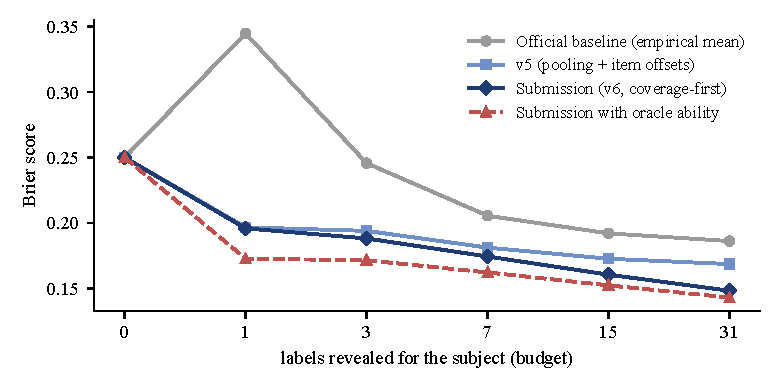
\includegraphics[width=0.7\linewidth]{fig_budget.pdf}
\caption{Brier score by budget on the 300-item regime. The oracle line replaces the estimated ability of each subject with its true accuracy on the benchmark.}
\label{fig:budget}
\end{figure}

\section{Online runs}
\label{app:runs}

\begin{table}[h]
\centering
\caption{Every online formative run in Table~\ref{tab:online}. $B_{31}$ is the mean Brier at budget 31, the draw's difficulty level.}
\small
\begin{tabular}{llcccc}
\toprule
Submission & Version & Pairs & Raw ALC & $B_{31}$ & Excess \\
\midrule
1016627 & v6 & 9 & 0.158 & 0.116 & 0.042 \\
1016628 & v6 & 9 & 0.170 & 0.143 & 0.027 \\
1016651 & v6, no API key & 8 & 0.158 & 0.134 & 0.024 \\
1017498 & + subject prior (v19) & 9 & 0.169 & 0.164 & 0.006 \\
1017499 & + subject prior (v19) & 9 & 0.159 & 0.151 & 0.008 \\
1017545 & + subject prior (v23) & 8 & 0.195 & 0.183 & 0.011 \\
1017562 & + subject prior (v25) & 8 & 0.179 & 0.169 & 0.010 \\
1017629 & + subject prior (v27) & 9 & 0.184 & 0.167 & 0.017 \\
1017607 & final & 8 & 0.181 & 0.175 & 0.006 \\
1017628 & final & 9 & 0.130 & 0.126 & 0.004 \\
1017682 & final (selected) & 9 & 0.164 & 0.149 & 0.014 \\
\bottomrule
\end{tabular}
\end{table}

\section{Variants that did not improve the submission}
\label{app:neg}

\begin{table}[h]
\centering
\caption{Variants tried and dropped. Differences in pair-averaged Brier ALC against the predictor of the same stage (negative is better).}
\label{tab:neg}
\footnotesize
\begin{tabular}{ll}
\toprule
Variant & Result \\
\midrule
Online Rasch model instead of shrinkage (v7, two seeds) & $-0.0001$ / $+0.0012$ \\
Multi-dimensional item ratings (v8) & $+0.0010$ ($+0.004$ online scale) \\
Staged acquisition, ability first & $+0.0021$ \\
Acquisition stratified by predicted difficulty & $+0.0013 \pm 0.0012$ \\
Haiku answer agreement (v31, online) & adj. $-0.011$ to $-0.014$ vs $-0.022$ \\
Opus and GPT prior averaged (simulation) & $-0.0011 \pm 0.0003$ \\
\quad same, online (4 runs) & $B_0$ excess 0.048--0.085 vs 0.031--0.049 \\
Text-learned difficulty (n-grams, embeddings, LoRA) & correlation $\le 0.08$ \\
Prior ensembles (Opus twice, Opus with Sonnet) & RMSE 0.139--0.142 vs 0.141 \\
Uncertainty sampling as in BLE (prior off) & $+0.0076 \pm 0.0015$ \\
Gemini added to the Opus and GPT prior & RMSE 0.137 vs 0.138 \\
GPT item ratings averaged with Opus & Brier 0.1391 vs 0.1387 \\
Task extraction for ratings (\texttt{clasheval}) & rank correlation 0.005 vs 0.10 \\
\bottomrule
\end{tabular}
\end{table}

\end{document}
